\documentclass[12pt]{tdtp}
\usepackage{tabularx,colortbl}
\usepackage{multirow}
\usepackage{listings}
\lstset{
	language=VHDL,
basicstyle=\tiny\ttfamily}
\definecolor{light-gray}{gray}{0.96}
\definecolor{pageheading-gray}{gray}{0.2}
\definecolor{dark-gray}{gray}{0.45}
\definecolor{dark-green}{rgb}{0.245,0.121,0.0}

\newcommand{\auteur}{Cedric Lemaitre}
\newcommand{\couriel}{c.lemaitre58@gmail.com}
\newcommand{\promo}{Bachelor in Computer Vision}
\newcommand{\annee}{2016-2017}
\newcommand{\matiere}{Digital Electronics}

\newcommand{\tdtp}{Labs 3}
\renewcommand{\sujet}{VHDL Design}


\begin{document}
\titre
We propose in this labs some advanced examples of component to design in VHDL.\\

\textit {NB : all examples should be check using \textbf{test-benchs} and simulatuon tools}


%%%%%%%%%%%%
\Exo

Create a multiplexer (mux) with :

\begin{enumerate}
	\item 2 inputs : data(8),add(3)
	\item 1 output : s(1)
	\item 1 CLK for synchronous
\end{enumerate}

\textit{NB : In electronics, a multiplexer (or mux) is a device that selects one of several analog or digital input signals and forwards the selected input into a single line. A multiplexer of $2^n$ inputs has $n$ select lines, which are used to select which input line to send to the output. A multiplexer is also called a data selector.}
%%%%%%%%%%%%
\newpage
\Exo
Create a VHDL Design that allow the same behavior of the common-cathoded BCD-decoder (figure : \ref{74HS48}) 74LS48 component\footnote{\url{http://pdf.datasheetcatalog.com/datasheet/motorola/74LS48.pdf}}. BCD-decoder is used to display value on 7-segment display (see figure : \ref{7seg}).\\
\\

\begin{figure}[h!]
\begin{center}
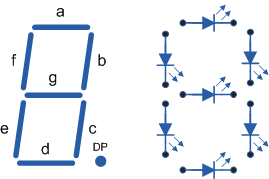
\includegraphics[scale=0.5]{images/7seg.png}
\caption{Example of 7 segments display}
\label{7seg}
\end{center}
\end{figure}


\begin{figure}[h!]
\begin{center}
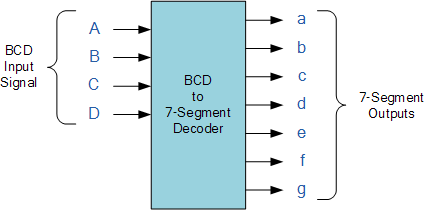
\includegraphics[scale=0.5]{images/74LS48.png}
\caption{BCD-decoder}
\label{74HS48}
\end{center}
\end{figure}

\textit{NB : 7-segment LED (Light Emitting Diode) or LCD (Liquid Crystal Display) type displays, provide a very convenient way of displaying information or digital data in the form of numbers, letters or even alpha-numerical characters.\\
Typically 7-segment displays consist of seven individual coloured LED’s (called the segments), within one single display package. In order to produce the required numbers or HEX characters from 0 to 9 and A to F respectively, on the display the correct combination of LED segments need to be illuminated and BCD to 7-segment Display Decoders.\\
A standard 7-segment LED display generally has 8 input connections, one for each LED segment and one that acts as a common terminal or connection for all the internal display segments. Some single displays have also have an additional input pin to display a decimal point in their lower right or left hand corner.}

%%%%%%%%%%%%
\newpage
\Exo

Create the state-machine represented of the following pictures (figure : \ref{fsm_seq_detector}) :\\
\\


\begin{figure}[h!]
\begin{center}
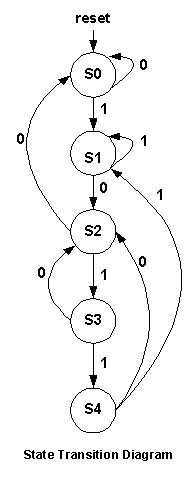
\includegraphics[scale=0.7]{images/fsm_seq_detector.png}
\caption{State machine}
\label{fsm_seq_detector}
\end{center}
\end{figure}

\textit{NB : A finite-state machine (FSM) or finite-state automaton (FSA, plural: automata), finite automaton, or simply a state machine, is a mathematical model of computation. It is an abstract machine that can be in exactly one of a finite number of states at any given time. The FSM can change from one state to another in response to some external inputs; the change from one state to another is called a transition. A FSM is defined by a list of its states, its initial state, and the conditions for each transition.\\
The behavior of state machines can be observed in many devices in modern society that perform a predetermined sequence of actions depending on a sequence of events with which they are presented. Examples are vending machines, which dispense products when the proper combination of coins is deposited, elevators, whose sequence of stops is determined by the floors requested by riders, traffic lights, which change sequence when cars are waiting, and combination locks, which require the input of combination numbers in the proper order.}
%%%%%%%%%%%

\end{document}
